% Created 2023-04-11 Tue 12:38
% Intended LaTeX compiler: pdflatex
\documentclass[14pt]{extarticle}
\usepackage[utf8]{inputenc}
\usepackage[T2A]{fontenc}
\usepackage{graphicx}
\usepackage{longtable}
\usepackage{wrapfig}
\usepackage{rotating}
\usepackage[normalem]{ulem}
\usepackage{amsmath}
\usepackage{amssymb}
\usepackage{capt-of}
\usepackage{hyperref}
\usepackage[russian]{babel}
\usepackage{tempora}
\usepackage{geometry}
\geometry{a4paper, left=30mm, top=20mm, bottom=20mm, right=15mm }
\usepackage{graphicx}
\usepackage{array}
\usepackage{tabularx}
\usepackage{listings}
\usepackage{float}
\usepackage{setspace}
\usepackage{tabularx}
\usepackage{longtable}
\usepackage{titlesec}
\titleformat*{\section}{\large\bfseries}
\titleformat*{\subsection}{\normalsize\bfseries}
\titleformat*{\subsubsection}{\normalsize\bfseries}
\addto\captionsrussian{\renewcommand{\contentsname}{\centering \normalsize СОДЕРЖАНИЕ}}
\addtocontents{toc}{\protect\thispagestyle{empty}}
\usepackage{titletoc}
\titlecontents{section}[0pt]{}{\contentsmargin{0pt} \thecontentslabel\enspace}{\contentsmargin{0pt}}{\titlerule*[0.5pc]{.}\contentspage}[]
\dottedcontents{subsection}[3.1em]{}{1.5em}{0.5pc}
\usepackage{caption}
\DeclareCaptionLabelSeparator{custom}{ -- }
\captionsetup[figure]{name=Рисунок, labelsep=custom, font={onehalfspacing}, justification=centering}
\usepackage{ragged2e}
\justifying
\setlength\parindent{1.25cm}
\sloppy
\usepackage{indentfirst}
\usepackage{multirow}
\usepackage{lscape}
\author{Панков Вася}
\date{\today}
\title{МДК 01.04 Системное программирование}
\hypersetup{
 pdfauthor={Панков Вася},
 pdftitle={МДК 01.04 Системное программирование},
 pdfkeywords={},
 pdfsubject={М. Ю. Кафтан},
 pdfcreator={Emacs 30.0.50 (Org mode 9.6.2)}, 
 pdflang={Russian}}

% Setup for code blocks [1/2]

\usepackage{fvextra}

\fvset{%
  commandchars=\\\{\},
  highlightcolor=white!95!black!80!blue,
  breaklines=true,
  breaksymbol=\color{white!60!black}\tiny\ensuremath{\hookrightarrow}}

% Make line numbers smaller and grey.
\renewcommand\theFancyVerbLine{\footnotesize\color{black!40!white}\arabic{FancyVerbLine}}

\usepackage{xcolor}

% In case engrave-faces-latex-gen-preamble has not been run.
\providecolor{EfD}{HTML}{f7f7f7}
\providecolor{EFD}{HTML}{28292e}

% Define a Code environment to prettily wrap the fontified code.
\usepackage[breakable,xparse]{tcolorbox}
\DeclareTColorBox[]{Code}{o}%
{colback=EfD!98!EFD, colframe=EfD!95!EFD,
  fontupper=\footnotesize\setlength{\fboxsep}{0pt},
  colupper=EFD,
  IfNoValueTF={#1}%
  {boxsep=2pt, arc=2.5pt, outer arc=2.5pt,
    boxrule=0.5pt, left=2pt}%
  {boxsep=2.5pt, arc=0pt, outer arc=0pt,
    boxrule=0pt, leftrule=1.5pt, left=0.5pt},
  right=2pt, top=1pt, bottom=0.5pt,
  breakable}

% Support listings with captions
\usepackage{float}
\floatstyle{plain}
\newfloat{listing}{htbp}{lst}
\newcommand{\listingsname}{Listing}
\floatname{listing}{\listingsname}
\newcommand{\listoflistingsname}{List of Listings}
\providecommand{\listoflistings}{\listof{listing}{\listoflistingsname}}


% Setup for code blocks [2/2]: syntax highlighting colors

\newcommand\efstrut{\vrule height 2.1ex depth 0.8ex width 0pt}
\definecolor{EFD}{HTML}{212121}
\definecolor{EfD}{HTML}{FAFAFA}
\newcommand{\EFD}[1]{\textcolor{EFD}{#1}} % default
\definecolor{EFh}{HTML}{607d8b}
\newcommand{\EFh}[1]{\textcolor{EFh}{#1}} % shadow
\definecolor{EFsc}{HTML}{4eee94}
\newcommand{\EFsc}[1]{\textcolor{EFsc}{#1}} % success
\definecolor{EFw}{HTML}{FF5722}
\newcommand{\EFw}[1]{\textcolor{EFw}{#1}} % warning
\definecolor{EFe}{HTML}{B71C1C}
\newcommand{\EFe}[1]{\textcolor{EFe}{#1}} % error
\definecolor{EFc}{HTML}{607d8b}
\newcommand{\EFc}[1]{\textcolor{EFc}{#1}} % font-lock-comment-face
\definecolor{EFcd}{HTML}{607d8b}
\newcommand{\EFcd}[1]{\textcolor{EFcd}{#1}} % font-lock-comment-delimiter-face
\definecolor{EFs}{HTML}{689f38}
\newcommand{\EFs}[1]{\textcolor{EFs}{#1}} % font-lock-string-face
\definecolor{EFd}{HTML}{673ab7}
\newcommand{\EFd}[1]{\textcolor{EFd}{#1}} % font-lock-doc-face
\definecolor{EFm}{HTML}{558b2f}
\newcommand{\EFm}[1]{\textcolor{EFm}{#1}} % font-lock-doc-markup-face
\definecolor{EFk}{HTML}{00796b}
\newcommand{\EFk}[1]{\textcolor{EFk}{#1}} % font-lock-keyword-face
\definecolor{EFb}{HTML}{B71C1C}
\newcommand{\EFb}[1]{\textcolor{EFb}{#1}} % font-lock-builtin-face
\definecolor{EFf}{HTML}{0097A7}
\newcommand{\EFf}[1]{\textcolor{EFf}{#1}} % font-lock-function-name-face
\definecolor{EFv}{HTML}{EF6C00}
\newcommand{\EFv}[1]{\textcolor{EFv}{#1}} % font-lock-variable-name-face
\definecolor{EFt}{HTML}{0097A7}
\newcommand{\EFt}[1]{\textcolor{EFt}{#1}} % font-lock-type-face
\definecolor{EFo}{HTML}{558b2f}
\newcommand{\EFo}[1]{\textcolor{EFo}{#1}} % font-lock-constant-face
\definecolor{EFwr}{HTML}{B71C1C}
\newcommand{\EFwr}[1]{\textcolor{EFwr}{\textbf{#1}}} % font-lock-warning-face
\definecolor{EFnc}{HTML}{2196f3}
\newcommand{\EFnc}[1]{\textcolor{EFnc}{#1}} % font-lock-negation-char-face
\definecolor{EFpp}{HTML}{FFA000}
\newcommand{\EFpp}[1]{\textcolor{EFpp}{#1}} % font-lock-preprocessor-face
\definecolor{EFrc}{HTML}{4527A0}
\newcommand{\EFrc}[1]{\textcolor{EFrc}{#1}} % font-lock-regexp-grouping-construct
\definecolor{EFrb}{HTML}{FFA000}
\newcommand{\EFrb}[1]{\textcolor{EFrb}{#1}} % font-lock-regexp-grouping-backslash
\definecolor{Efob}{HTML}{EFEBE9}
\newcommand{\EFob}[1]{\colorbox{Efob}{\efstrut{}#1}} % org-block
\newcommand{\EFhn}[1]{#1} % highlight-numbers-number
\newcommand{\EFhq}[1]{#1} % highlight-quoted-quote
\newcommand{\EFhs}[1]{#1} % highlight-quoted-symbol
\newcommand{\EFrda}[1]{#1} % rainbow-delimiters-depth-1-face
\newcommand{\EFrdb}[1]{#1} % rainbow-delimiters-depth-2-face
\newcommand{\EFrdc}[1]{#1} % rainbow-delimiters-depth-3-face
\newcommand{\EFrdd}[1]{#1} % rainbow-delimiters-depth-4-face
\newcommand{\EFrde}[1]{#1} % rainbow-delimiters-depth-5-face
\newcommand{\EFrdf}[1]{#1} % rainbow-delimiters-depth-6-face
\newcommand{\EFrdg}[1]{#1} % rainbow-delimiters-depth-7-face
\newcommand{\EFrdh}[1]{#1} % rainbow-delimiters-depth-8-face
\newcommand{\EFrdi}[1]{#1} % rainbow-delimiters-depth-9-face
\begin{document}

\begin{titlepage}

\centering{ГУАП}

\vspace{32pt}

\centering{ФАКУЛЬТЕТ СРЕДНЕГО ПРОФЕССИОНАЛЬНОГО ОБРАЗОВАНИЯ}

\vspace{60pt}

\raggedright{ОТЧЕТ \\
ЗАЩИЩЕН С ОЦЕНКОЙ}
\vspace{14pt}

\raggedright{ПРЕПОДАВАТЕЛЬ}

\vspace{12pt}

\begin{tabularx}{\textwidth}{ >{\centering\arraybackslash}X >{\centering\arraybackslash}X >{\centering\arraybackslash}X }
	 преподаватель & & М. Ю. Кафтан \\ 
	 \hrulefill & \hrulefill & \hrulefill \\ 
\footnotesize{должность, уч. степень, звание} & \footnotesize{подпись, дата} & \footnotesize{инициалы, фамилия} \\ 
\end{tabularx} 
 
\vspace{48pt} 

\centering{ОТЧЕТЫ О ЛАБОРАТОРНЫХ РАБОТАХ} 

\vspace{76pt} 

\centering{По дисциплине: МДК 01.04 Системное программирование} 

\vspace*{\fill} 

\raggedright{РАБОТУ ВЫПОЛНИЛ} 

\vspace{10pt} 

\begin{tabularx}{\textwidth}{>{\raggedright\arraybackslash}X  >{\centering\arraybackslash}X >{\centering\arraybackslash}X >{\centering\arraybackslash}X }
	 СТУДЕНТ ГР. № & 021к & & Панков Вася \\ 
	 & \hrulefill & \hrulefill & \hrulefill \\ 
	 &  & \footnotesize{подпись, дата} & \footnotesize{инициалы, фамилия} \\ 
\end{tabularx} 
 
\vspace*{\fill} 

\centering{Санкт-Петербург \the\year} 

\end{titlepage}

\tableofcontents \clearpage

\section{Лабораторная работа № 4}
\label{sec:org27c83b4}

Тема: Анализ работы микропроцессора при выполнении линейной программы.

Цель работы:
\begin{itemize}
\item освоить приемы программирования на языке Ассемблера (Ass) по моделированию
\end{itemize}
работы микропроцессорной системы при выполнении линейных программ.

Индивидуальное задание:


Разработать линейную программу на языке Ассемблера МП КР580 для нахождения
значения функции и определить время, затрачиваемое на выполнение программы
(составить алгоритм, определить области размещения программы и данных,
написать программу в мнемонических кодах с комментариями, проверить правильность выполнения алгоритма).


$$ Z = (X1 + \neg Y1) + (\neg X2 + Y2) $$

Начальный адрес программы: 0109H

Начальный адрес памяти: 0209H


\begin{longtable}{|l|l|l|}
\hline
Адрес ячейки памяти & Содержимое ячейки памяти & Комментарий\\[0pt]
\hline
\endfirsthead
\multicolumn{3}{l}{Продолжение с предыдущей страницы} \\[0pt]
\hline

Адрес ячейки памяти & Содержимое ячейки памяти & Комментарий \\[0pt]

\hline
\endhead
\hline\multicolumn{3}{r}{Продолжение на следующей странице} \\
\endfoot
\endlastfoot
\hline
0209H & 0005H & Y1\\[0pt]
\hline
020AH & 000CH & X1\\[0pt]
\hline
020BH & 0017H & X2\\[0pt]
\hline
020CH & 0055H & Y2\\[0pt]
\hline
020DH & 003DH & Результат\\[0pt]
 &  & выполнения программы\\[0pt]
\hline
\end{longtable}

\begin{Code}
\begin{Verbatim}
\color{EFD}\EFf{LXI} \EFk{H},0209\EFcd{;}
\EFf{MOV} \EFk{A},M\EFcd{;}
\EFf{CMA}\EFcd{;}
\EFf{INX} \EFk{H}\EFcd{;}
\EFf{ADD} \EFk{M}\EFcd{;}
\EFf{MOV} \EFk{D},A\EFcd{;}
\EFf{INX} \EFk{H}\EFcd{;}
\EFf{MOV} \EFk{A},M\EFcd{;}
\EFf{CMA}\EFcd{;}
\EFf{INX} \EFk{H}\EFcd{;}
\EFf{ADD} \EFk{M}\EFcd{;}
\EFf{ADD} \EFk{D}\EFcd{;}
\EFf{INX} \EFk{H}\EFcd{;}
\EFf{MOV} \EFk{M},A\EFcd{;}
\EFf{RST} \EFk{07}\EFcd{;}
\end{Verbatim}
\end{Code}


В эмуляторе:

\begin{figure}[H]
\centering
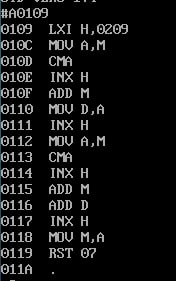
\includegraphics[width=.9\linewidth]{images/2023-04-11_12-30-04_screenshot.png}
\caption{Ввод программы в эмулятор}
\end{figure}



\begin{figure}[H]
\centering
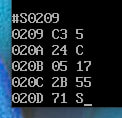
\includegraphics[width=.9\linewidth]{images/2023-04-11_12-30-46_screenshot.png}
\caption{Ввод данных}
\end{figure}

\begin{figure}[H]
\centering
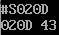
\includegraphics[width=.9\linewidth]{images/2023-04-11_12-31-25_screenshot.png}
\caption{Результат выполнения}
\end{figure}
\end{document}